\documentclass{article}
\usepackage[italian]{babel}
\usepackage[T1]{fontenc}
\usepackage{graphicx}
\usepackage[utf8x]{inputenc}
\usepackage{amsmath}
\usepackage{amsthm}
\usepackage{hyperref}
\usepackage{caption}
\date{}
\author{Gruppo 1G.BT \\ Francesco Sacco Lorenzo Cavuoti}
\title{Caratteristiche porte logiche e semplici circuiti logici}

\begin{document}

\maketitle
\paragraph{2)}
	\subparagraph{a.} Si è montato un flip-flop D-Latch usando le porte NAND dell'integrato SN74LS00 come in figura \ref{fig:d-latch}, l'ingresso EN è stato collegato ad un terminale di un DIP Switch con l'altro estremo messo a terra, mentre l'ingresso D è stato collegato all'uscita TTL del generatore di funzioni con $f\approx1$Hz.
	\subparagraph{b.} Si è ottenuta la tabella di verità \ref{tab:d-latch}, in accordo con le aspettative, inoltre si è misurato il ritardo tra l'ingresso D e l'uscita Q: $t_{pLH}=27.3\pm0.9 ns$ $t_{pHL}=63\pm3 ns$ dove l'errore è dato dalla difficoltà di misura del tempo in quanto i segnali erano frastagliati. Considerando che il segnale in ingresso attraversa 3 porte NAND i tempi sono in accordo con quelli del datasheet dell'integrato.
	\subparagraph{c.} Abbiamo verificato che l'ingresso ENABLE è di predefinito attivo alto\newline
	
	\begin{minipage}{.6\linewidth}
		\centering
		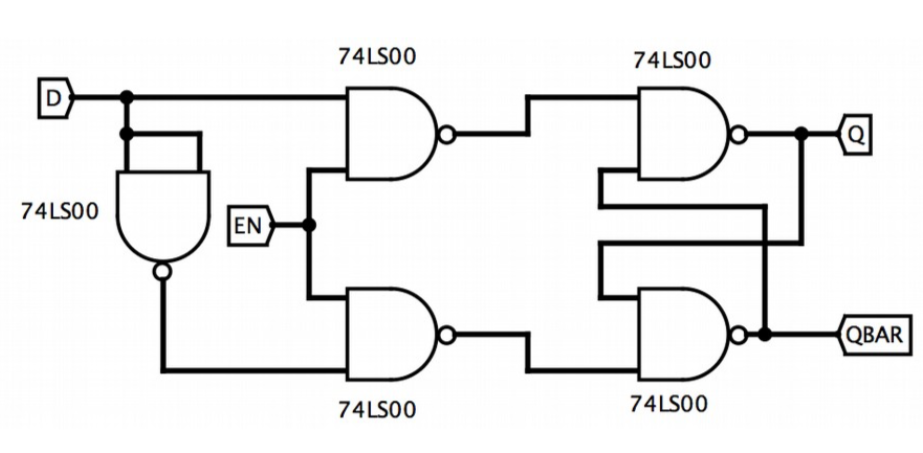
\includegraphics[width=\linewidth]{immagini/dlach}
		\captionof{figure}{Flip-flop D-latch}
		\label{fig:d-latch}
	\end{minipage}
	\begin{minipage}{.4\linewidth}
		\begin{tabular}{cccc}
\hline
	EN & D & Q & !Q\\ 
\hline
	$0$ & X & $Q_{n-1}$ & $!Q_{n-1}$ \\
	$1$ & $0$ & $0$ & $1$ \\
	$1$ & $1$ & $1$ & $0$ \\
\hline
\end{tabular}

		\captionof{table}{Tabella di verità del flip-flop D-latch}
		\label{tab:d-latch}
	\end{minipage}\newline

\paragraph{3)}
	\subparagraph{a.} Abbiamo montato il divisore in frequenza come nell'immagine, \ref{fig:div_freq1}, le resistenze ($330\Omega$ nominali) sono state utilizzate per limitare la corrente che passa nei led.
	\subparagraph{b.} Si è inviato un clock a circa 1Hz e abbiamo verificato che il circuito sia effettivamente un contatore da 0 a 15 in codifica binaria.
	\subparagraph{c.} Abbiamo inviato un segnale di clock a $80.7\pm0.3$kHz e verificato che le uscite dividono il segnale. Sotto sono fornite le immagini dei segnali visti all'oscilloscopio, in tutte le immagini il segnale di clock è posizionato in basso mentre l'uscita in alto.\newline
	I tempi di sfasamento da LOW a HIGH per ciascuna uscita sono: $t_{pLH} Q_0=20.0\pm0.9ns \quad t_{pLH} Q_1=18.0\pm0.9ns \quad t_{pLH} Q_2=17.0\pm0.9ns \quad t_{pLH} Q_3=17.0\pm0.9ns$. Siccome il segnale era frastagliato la stima degli errori è stata effettuata considerando l'incertezza nel determinare la posizione di $V=V_{max}/2$. Notiamo infine che i tempi di sfasamento delle uscite sono molto simili tra loro, questo è in accordo con il fatto che abbiamo utilizzato un contatore sincrono.
	%la stima degli errori è stata effettuata considerando il valore massimo e quello minimo per cui lo sfasamento è notabile e facendo la media e la somma dimezzata. (non so spiegarlo decentemente lorenzo aiuto!)\newline
	
	\begin{figure}
	\begin{center}
		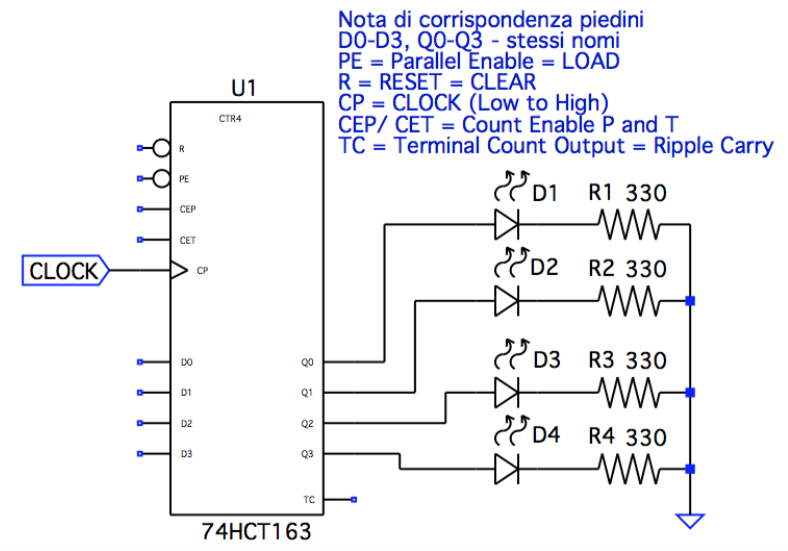
\includegraphics[width=0.7\linewidth]{immagini/div_freq1}
		\captionof{figure}{Schema circuitale del divisore di frequenza}
		\label{fig:div_freq1}
	\end{center}
	\end{figure}

	\begin{minipage}{.5\linewidth}
		\centering
		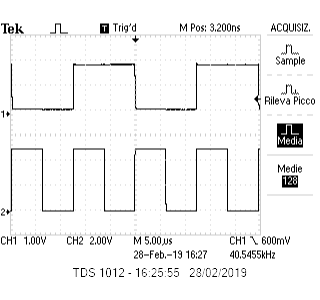
\includegraphics[width=\linewidth]{immagini/f1_2}
		\captionof{figure}{$Q_0$}
		\label{fig:f1_2}
	\end{minipage}
	\begin{minipage}{.5\linewidth}
		\centering
		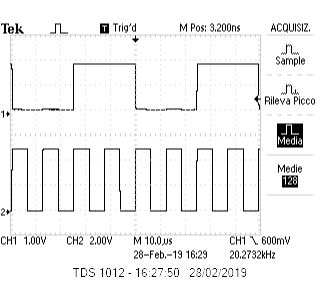
\includegraphics[width=\linewidth]{immagini/f1_4}
		\captionof{figure}{$Q_1$}
		\label{fig:f1_4}
	\end{minipage}\newline
	\begin{minipage}{.5\linewidth}
		\centering
		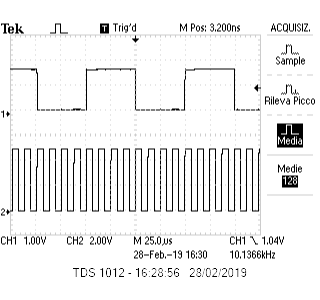
\includegraphics[width=\linewidth]{immagini/f1_8}
		\captionof{figure}{$Q_2$}
		\label{fig:f1_8}
	\end{minipage}
	\begin{minipage}{.5\linewidth}
		\centering
		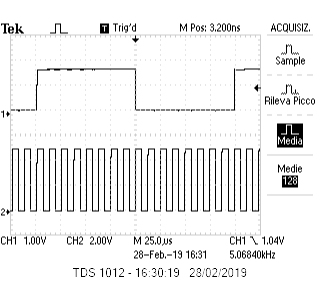
\includegraphics[width=\linewidth]{immagini/f1_16}
		\captionof{figure}{$Q_3$}
		\label{fig:f1_16}
	\end{minipage}\newline\newline

	\subparagraph{d.} Quando il contatore arriva a 9 si ha che $(Q_0,Q_1,Q_2,Q_3)=(1,0,0,1)$, in particolare esso è il primo numero che ha sia la porta $Q_0$ che $Q_3$ sono HIGH, quindi questa condizione può essere usata per resettare il contatore. Essendo di defaut la porta di RESET HIGH basta collegare al RESET l'uscita di un NAND che ha come ingressi $Q_0$ e $Q_3$. Il segnale dell'uscita $Q_0$ vista all'oscilloscopio è mostrato in figura \ref{fig:3d}
		\begin{figure}
		\begin{center}
			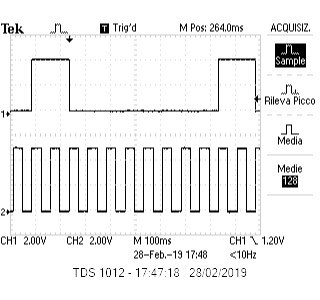
\includegraphics[width=0.5\linewidth]{immagini/3d}
			\captionof{figure}{Contatore decimale}
			\label{fig:3d}
		\end{center}
		\end{figure}

	\paragraph{4)}
	\subparagraph{a.} Abbiamo costruito uno shift register a 4 bit utilizzando 2 integrati 74LS74 contenenti 2 D-Latch ciascuno \ref{fig:circuito4}. L'ingresso di Preset è stato collegato ad un pulsante con l'altro estremo messo a terra mentre l'ingresso D è stato collegato al DIP Switch, sempre con l'altro estremo messo a terra. Le uscite $Q_0,Q_1,Q_2,Q_3$ sono state collegate a dei LED con una resistenza verso terra di $330\Omega$ nominali. Infine si è inviato un segnale di clock a circa 1Hz preso dall'uscita TTL del generatore di funzioni. Si osserva che il circuito propaga il segnale d'ingresso D su ciascuno dei D-Latch con un tempo di propagazione da uno all'altro pari a $1/f_{clock}$, in pratica il circuito mantiene la memoria del segnale in ingresso e dei segnali presenti all'ingresso fino a 3 cicli di clock prima; equivalentemente si può dire che ad ogni ciclo di clock il segnale in ingresso viene memorizzato nel D-Latch successivo (infatti l'uscita di ciascun D-Latch è collegata all'entrata di un altro) fino ad arrivare all'ultimo D-Latch dove viene perso.
	\subparagraph{b.} Dopo aver premuto il pulsante di preset lo stato delle uscite è alto, LED acceso.
	\subparagraph{c.} Si è collegata l'uscita $\ Q_{3}$ all'entrata D del primo D-Latch scollegando il DIP Switch, la frequenza di clock è stata alzata a circa 10Hz. Si osserva che partendo da un segnale D alto questo inizialmente viene propagato come nel circuito precedente, illuminando tutti i led, però quando l'ultimo led viene acceso si ha $Q_{3}=1$ e $!Q_{3}=0$, quindi nel ciclo di clock successivo D è basso il che fa spegnere tutti i led. Quando l'ultimo led si spegne si ha $Q_{3}=0$ e $!Q_{3}=1$, il quale porta D ad essere alto, ritornando alle condizioni iniziali. Quindi il circuito esegue il ciclo spiegato sopra continuamente fino a che gli viene fornita corrente, di conseguenza ci aspettiamo che sui piedini di uscita si presenti una frequenza $f=1/8f_{clock}$ come si osserva all'oscilloscopio figura \ref{fig:punto4}.
	
	
\begin{figure}
	\centering
	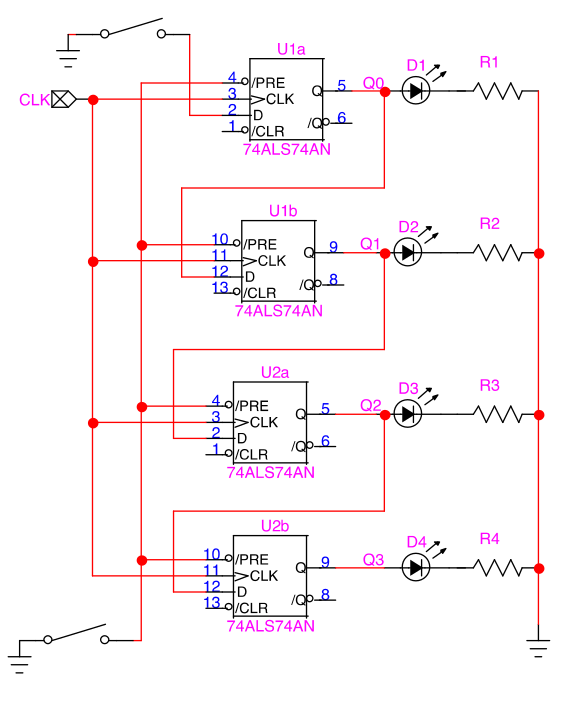
\includegraphics[width=0.7\linewidth]{immagini/circuito4}
	\caption{Circuito utilizzato nel punto 4}
	\label{fig:circuito4}
\end{figure}

\begin{figure}
	\centering
	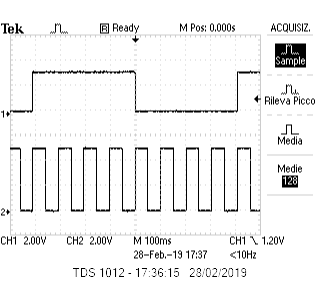
\includegraphics[width=0.7\linewidth]{immagini/punto_4}
	\caption{In basso: segnale di clock. In alto: segnale all'uscita dei D-Latch}
	\label{fig:punto4}
\end{figure}


\end{document}